\section{Solution Proposal} \label{solution}
\subsection{Technical Literature Review}
In order to best understand the problem and ensure the proposed solution is not a retread of existing work, a preliminary literature review is necessary.

The most directly related existing work is the 2013 paper \textit{Modeling and Control of Casterboard Robot} from the 9th IFAC Symposium on Nonlinear Control Systems, which outlines the design, modelling and prototypying of a robot propelled by the mechanics of the Ripstik \cite{CasterboardRobot}. While this covers many similar tasks to those defined in the problem description, the end goal is a casterboard robot rather than a mode of transportation, making the requirements of the control problem very different. Furthermore, the paper does not consider stability as part of the problem, using outriggers to balance the robot, which makes the initial model very different since it does not consider the z-axis and makes significant assumptions about the angles of the foot platforms \cite{CasterboardRobot}.

Similar modelling and control work has also been done for bicycles \cite{BikeModel,BikeControl} which bear similarities in that they are both 2 wheeled vehicles that use nonholonomic constraints and Euler angles in their modelling \cite{BikeModel}. These may also provide some reference in terms of overall direction and approach for the project.
\subsection{Overview}
As required by the problem description, the intent is to develop a complete working mathematical model of the Ripstik, a method of visualizing the model outputs on a 3D representation of the Ripstik (to analyze and present results), and a control law for the system. Additionally, accompanying research will be done to examine the feasibility of a self-balancing, self-propelled electric Ripstik as a commercial product and determine whether it is viable or useful from a technical perspective.
\subsection{Tools}
\subsubsection{Mathematica}

Mathematica is a powerful tool with a comprehensive set of built in functions \cite{Wolfram}. Modeling the Ripstik will require extensive symbolic (Lagrangian) equations. Mathematica has the ability to support these equations, and efficiently compute the solutions to the equations in a precise manner \cite{Wolfram}. This reduces the possibility of human error when developing the equations and minimizes computation time.

In order to minimize the possibility of errors in the code and ensure readability throughout, all code will be reviewed by another group member once complete. Additionally, symbolic variables and functions will be given useful, descriptive names and code will include comments where necessary.
\subsubsection{Three.js}
Three.js is a powerful Javascript library designed to facilitate 3D rendering in web browsers using WebGL (Web Graphics Library) \cite{threejs}. This will be used for producing the 3D visualization of the model results in a web browser. This eliminates the need for powerful hardware or locally installed software for the 3D animation, allowing results to be quickly checked from any device. Additionally, three.js is widely used by industry leaders \cite{threejs} and should be easily implemented, minimizing the resources that need to be allocated to the task since it is not part of the core mathematical model.

\subsection{Mathematical Fundamentals} \label{solutionMath}

The initial focus for developing a mathematical model of the Ripstik was placed on determining the number of degrees of freedom in the system. A coordinate system was defined, assumptions were made, and Euler angles were applied to said coordinate system so that all constraints could be clearly defined.
\par
The body-fixed coordinate system used for the caster board can be seen in Figure \ref{fig:Coordinate_System}. The origin of this coordinate system will be placed at the center of the torsion bar. The \textit{x-y} plane will be parallel with the surface of the Ripstik deck platforms when no torsion is applied with the \textit{x} axis in the direction of the torsion bar, \textit{+x} pointing towards the kick nose and the \textit{y} axis perpendicular. The \textit{z} axis will be normal to this plane, with \textit{+z} pointing upwards. \textit{y} axis direction is defined by the right hand rule. The inertial coordinate system is defined with the  \textit{x'-y'-z'} axes which are initially coincident with the body fixed system but remain stationary.
\begin{figure}[!htb]
\centering
\minipage{0.3\textwidth}
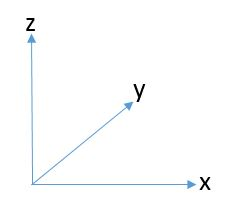
\includegraphics[width=\linewidth]{Coordinate_System.JPG}
\caption{Coordinate System developed for modeling of Ripstik}\label{fig:Coordinate_System}
\endminipage
\end{figure}
\par
As previously stated, a number of assumptions will need to be made in order to facilitate modelling the Ripstik. The wheels of the Ripstik are assumed to roll without slipping \cite{CasterboardRobot,BikeModel}. However, unlike in previous work \cite{CasterboardRobot}, it is assumed that the Ripstik will be capable of moving in all 3 axes of the global coordinate system since balance is a central component of the control problem.
\par
Euler angles were implemented into the system to represent the roll, pitch, and yaw of the Ripstik. The roll, pitch, and yaw were represented by $\alpha, \psi$, and $\theta$ respectively.
\par
The yaw angle $(\theta)$ was represented by a moment taken around the \textit{z'}-axis (right hand rule applied). The angle $\theta$ is taken between the {x} and \textit{x'}-axes. A graphical representation of the yaw angle can be seen in Figure \ref{fig:Yaw_angle}.
\begin{figure}[!htb]
\centering
\minipage{0.3\textwidth}
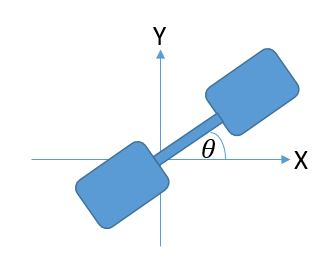
\includegraphics[width=\linewidth]{Yaw_angle.JPG}
\caption{Yaw angle $\theta$ about the z axis}\label{fig:Yaw_angle}
\endminipage
\end{figure}   
\par
The roll angles $\alpha$ describe the rotation of the deck platforms about the {x}-axis. There will be two roll angles on the Ripstik, the first on the front platform ($\alpha_f$) and the second on the rear platform ($\alpha_r$). A graphical representation of the roll angles can be seen in Figure \ref{fig:Roll_angle}.
\begin{figure}[!htb]
\centering
\minipage{0.3\textwidth}
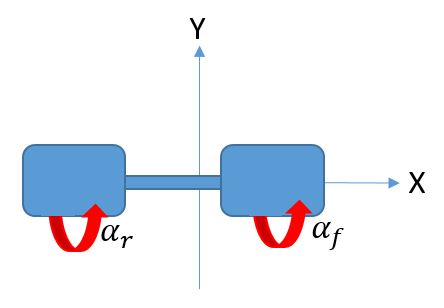
\includegraphics[width=\linewidth]{Roll_angle.JPG}
\caption{Roll angle $\theta$ about the x axis}\label{fig:Roll_angle}
\endminipage
\end{figure}
\par
The pitch angle $\psi$ is the angle that the wheels make, intersecting a plane between the x and z axis. It is essential that the angle which the casters are oriented at is taken into consideration, and will be represented by $\beta$. The wheels are completely unbounded in their ability to rotate, and can pivot through [0,2$\pi$]. There will be two pitch angles on the Ripstik, the first on the front caster ($\psi_f$) and the second on the rear caster ($\psi_r$). A graphical representation of the pitch angles can be seen in Figure \ref{fig:Pitch_angle}.
\begin{figure}[!htb]
\centering
 \minipage{0.3\textwidth}
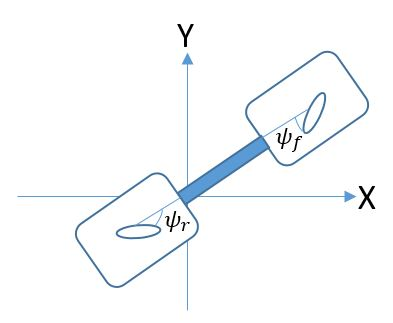
\includegraphics[width=\linewidth]{Pitch_angle.JPG}
\caption{Pitch angle $\theta$ measured relative to the body fixed axes}\label{fig:Pitch_angle}
\endminipage
\end{figure}
\par

The caster board system has eight degrees of freedom represented by  [x, y, z, $\theta$, $\psi_{f}$, $\psi_{r}$, $\alpha_{f}$, $\alpha_{r}$].

Lagrangian equations for the system have not yet been developed, however, assuming the wheels roll without slipping is a nonholonomic constraint \cite{CasterboardRobot,BikeModel} that will need to be considered. Further research and analysis will be required to accurately define this and other possible constraints \cite{Lewis,BikeModel}.

\subsection{Social Considerations}
\subsubsection{Rider Safety}
The most recent study of skateboard related trauma occurred in 2010 and focused on the last five years of data from the National Trauma Databank in the United States, further supporting the data with comparisons to other recent studies and analysis of datasets from outside sources \cite{Injury}. The study analyzed 2270 hospital patients admitted due to skateboarding related injuries. Of these, 8\% were under 10 years of age, 58\% were between 10 and 16 years of age, and the remaining 34\% were older than 16 \cite{Injury}. One statistic the researchers highlighted was the rate of incidence of traumatic brain injury among those admitted; in aforementioned age groups, these were 24.1\%, 32.6\%, and 45.5\% respectively\cite{Injury}. While the study concluded that ``helmet utilization and designated skateboard areas significantly reduce the incidence of serious head injuries'' \cite{Injury}, this also highlights the need to develop an electric Ripstik that will minimize the chance of rider injury and, if possible, reduce the severity of unavoidable falls. As the study suggests, proper protective equipment will also be crucial for any user of the proposed product. 

For the final Ripstik system, this means preventing the automated control from applying extreme acceleration that could cause the rider to be ejected from the board. Similarly, it should keep the board stable in all scenarios, preventing the rider from falling off the side during turns or at low speeds, when it is difficult to keep the board stable. These considerations will be directly addressed by evaluation criteria since they relate to the control law.
\subsubsection{Cybersecurity} \label{Cybersecurity}
With any digital system in the 21st century, cybersecurity is a key concern as it has grown far beyond simply protecting information or resources against intruders \cite{cybersecurity}. As electric skateboards have risen in popularity, they have attracted the attention of major hacking conferences. The most notable example was a recent presentation at DEF CON, ``the world's longest running and largest underground hacking conference'' \cite{DEFCONsite}, where a group demonstrated techniques for jamming and overriding the wireless control signals used by three popular electric skateboard brands, allowing them to adjust speed, apply the brakes, and permanently disable the vehicles \cite{DEFCON,wiredArticle}. This has direct implications for rider safety since a sudden stop at high speeds could cause significant injury. 

These developments must be considered for a commercial electric Ripstik product since some method of wireless speed control will likely be required to allow adequate control for the rider. The DEF CON presenters noted that proprietary RF (radio frequency) protocols were particularly easy to capture and replicate using SDR (software defined radio) \cite{Radio}\cite{DEFCON} but that more modern Bluetooth features could provide sufficient security to prevent hacking using current techniques \cite{DEFCON}. Possible technologies like these will be considered to provide a solution that minimizes potential cybersecurity threats.
\subsection{Environmental Considerations}
\subsubsection{Battery Technologies}
Modern electronic devices like the proposed electric Ripstik generally rely on rechargeable lithium-ion or lithium-polymer batteries due to their energy storage density and long product lives \cite{BatteryRecharge}. A life cycle analysis of these types of batteries revealed a high cost to the environment and to human health; high lead content (averaging 6.29 mg/L \cite{BatteryRecharge}) and cobalt content (averaging 163544 mg/kg \cite{BatteryRecharge}) both cause them to be classified as hazardous according to U.S. federal regulations \cite{BatteryRecharge}. There are risks of  resource depletion, detrimental effects to human health, and ecotoxicity associated with these battery technologies \cite{BatteryRecharge} which will have to be carefully considered when developing a solution. The potential and feasibility of next generation energy storage technologies like graphene batteries \cite{Graphene} will also be analyzed.

Batteries in personal electric transportation devices became a topic of conversation when the US government recalled over 500,000 two wheeled, self balancing scooters in 2016 due to a risk of batteries sparking, catching fire and exploding, causing at least 18 injuries \cite{CBCArticle}. This brings a clear social impact as well since there is a safety risk associated with low cost batteries manufactured in China\cite{CBCArticle}.
\subsubsection{Other Materials}
The current Ripstik products manufactured by Razor USA LLC feature plastic outer shells around a metal internal structure. The plastics pose a unique set of environmental challenges including greenhouse gas emissions, energy consumption and waste during production \cite{PlasticAssessment}. Further challenges occur at the disposal stage, particularly as the quantities of plastic increase. A 2013 article in the International Weekly Journal of Science argued that ``policies for managing plastic debris are outdated and threaten the health of people and wildlife'' \cite{Plastic} and that plastics should be classified as hazardous materials. The article mentions that 0.28 billion tonnes of plastic were produced in 2012 but projects that 33 billion tonnes could be produced in 2050 based on the current trends, posing a significant threat to animal food webs \cite{Plastic}. Additionally, over 78\% of the priority pollutants listed by the United States Environmental Protection Agency (EPA) stem from plastic \cite{Plastic}. These impacts must be taken into account when considering potential materials for the final design and should be weighed against other options.
\subsubsection{Commuting} \label{commuting}
Another potential benefit of a practical mode of medium distance (10-20 km range) electric transportation is the potential to reduce car usage since the electric Ripstik could serve as a replacement for or supplement to the consumer's current urban commute. In the United States, the Census Bureau reports that 75\% of commuters, or 105 million people, commuted alone by car, with only 5\% using public transit, 2.9\% walking, and 0.6\% traveling by bicycle \cite{harvard}. With the average commute being about 25 minutes \cite{harvard}, it is likely that many of the commuters currently traveling by car could benefit from a self propelled, electric transportation system, thereby reducing the emissions produced by cars. The EPA estimates that a typical passenger vehicle emits approximately 411 grams of carbon dioxide per mile, or 4.7 metric tons per year, which contributes to global warming, acid rain, and more \cite{EPA}.
\subsection{Economic Considerations}
The viability of the electric Ripstik for commuting, as discussed in subsection \ref{commuting}, presents a potential market as an electric transportation device; unfortunately, this is not a well established market and therefore does not have readily available data. Multiple recent articles and conferences quote this as being an ``emerging market'' \cite{emerging1,emerging2,emerging3}, indicating that there is significant growth and room for new companies and products to enter the space. This will be an area of particular interest going forward in the project since new data may emerge.

Additionally, the electric Ripstik could be established as a competitor to traditional skateboards, which currently have an estimated 11 million users in the United States and a global market size in excess of \$5 billion \cite{Skateboarding}.

The design of the Ripstik, specifically the ability to generate propulsion without removing feet from the board surface, will allow for the development of new tricks and skills by riders. This could allow for the electric Ripstik to be adopted by skateboard riders looking to expand their abilities. With the global skateboarding market being so large, a manufacturer could have the potential to generate significant sales if the board is adopted by even a small segment of current skateboard riders.
\subsection{Legal Considerations}
\subsubsection{Existing Patents}
The current Ripstik design and the proposed electric Ripstik are both affected by a number of existing patents that will have to be carefully read and addressed, either by licensing or avoiding infringement altogether. 

The main patent of note is the original caster board patent, titled \textit{Skateboard with direction-caster}, which details the two boards connected by ``an elastic member'' with casters on each platform \cite{directionCasterPatent}. This patent is directly referenced by a recent patent for a \textit{Casterboard}, which focuses on the ornamental design seen on modern Ripstik products \cite{casterboardPatent}.

Other relevant patents include a detailed filing for an \textit{Electric skateboard} that includes battery and motor mounting, drivetrain details, and board integrated wiring, all of which are relevant to an electric Ripstik \cite{electricSkateboardPatent}.
\subsubsection{Street Legality}
Since skateboards the original inspiration for the Ripstik, many of the laws currently applied to skateboards are likely to be imposed on Ripstiks. Preliminary research has already found laws prohibiting the use of skateboards on public streets in Toronto and Fredericton \cite{TOLaws}, which may limit the electric Ripstik's feasibility as a method of commuting in some cities.

Similarly, many cities have bans on certain forms of personal electric transportation. Notably, until Assembly Bill 2054 was presented in mid-2015 in California, a longstanding ban from 1977 made any motorized skateboard illegal since the powered skateboards of the day were gas-powered, noisy and dangerous \cite{OCLaws,WSJLaws}. Similar bans may still be in place elsewhere. Other relevant laws are those that were originally put in place to regulate the two-wheeled, self balancing electric scooters that rose to popularity in late 2015. One major manufacturer states that they have been banned from airlines in Canada and the USA and their usage is heavily restricted or banned in regions including Toronto, Vancouver, New York City, and the state of California \cite{leetboard}.
Further research will be necessary to fully examine the potential impact of existing laws.
\subsection{Evaluation}
\begin{center}
\textit{\textbf{Table 1:} Evaluation criteria for the project deliverables}
  \begin{tabular}{|p{2.3cm}|p{2.5cm}|p{4.5cm}|p{5.7cm}|}
    \hline
    \textbf{Deliverable} & \textbf{Functionality} & \textbf{Description} & \textbf{Test} \\ \hline
    Model & Parameters & All numerical parameters for the mathematical model must be configurable. Ex: angles of the casters, board dimensions, masses, etc. & The user can easily, through either single commands or a GUI, manipulate all constants. No values are hardcoded. \\
    \hline 
    Model & Inputs & Sufficient control inputs have been defined to allow for full control over the system. & The user can implement control functions in Mathematica that apply forces where control inputs may be of use without manipulating core model code. \\
    \hline
    Model & Outputs & Sufficient control outputs have been defined to fully describe Ripstik behaviour. & The user can easily retrieve output data for Ripstik behaviour that creates a complete represntation of behaviour in the visualization tool. \\
    \hline
    Model & Realism & Model output, when no control is applied, reflects real world behaviour of the system. & The user observes output that is comparable to behaviour observed on the test Ripstik with no rider. \\
    \hline Visualization & Accuracy & 3D animation output accurately reflects the model output based on provided input data. & A test data set, which cycles through allowable values for each model output, can be sent to the visualization tool and produces expected output. \\
    \hline Control \newline System & Board \newline Stability & The control system prevents the Ripstik from becoming destabilized, ejecting the rider & During testing, the Ripstik deck platforms do not reach an incline of over 20 degrees from the horizontal. \\
    \hline Control \newline System & Straight line tracking & The control system will be able to move the Ripstik straight & The Ripstik travels 10m straight ahead without deviating more that 0.2m from the path \\
    \hline Control \newline System & Turning & The control system will be able to turn the Ripstik & The Ripstik can traverse a complete circle of 1m radius both CW \& CCW without deviating more that 0.3m from the path \\
    \hline
    \end{tabular}
\end{center}
Note that tests criteria for the control system are based on current user experience with the Ripstik and are subject to change as the project develops.